\chapter{A Rewriting Logic Semantics for Probabilistic Event-B}
The rewriting logic approach to probabilistic Event-B \cite{Olarte}, introduces a method for translating probabilistic Event-B models to PMaude models that are executable in PVeStA. Formally speaking, it is a map $\llbracket \cdot \rrbracket: (\mathscr{C}, \mathscr{M}) \rightarrow \mathscr{R}_\mathscr{M}$ from a probabilistic event model to a rewrite theory. There are two main steps for this transformation:

\begin{enumerate}
    \item Specify a rewrite theory $\mathscr{R}$ to encode the static parts of the model, i.e. the context and the initialization of the machine.
    \item Then, $\mathscr{R}$ is extended with equations and rewrite rules that correspond to the events in the machine $\mathscr{M}$.
\end{enumerate}

The rewrite theory $\mathscr{R}$ works as a framework that allows to represent each one of the Event-B's elements inside Maude. To explore the implementation of it, the reader can refer to \cite{tool.website}, where the rewrite theory is specified with multiple Maude system modules in the folder named as \texttt{m-theory}. For the sake of simplicity, a general definition of $\mathscr{R}$ will be given.

$\mathscr{R}$ consists of four Maude system modules: \texttt{SAMPLER}, \texttt{EB-CORE}, \texttt{EBCONTEXT}, and \texttt{EBMACHINE}. \texttt{SAMPLER} contains the definition of functions for probabilistic sampling. \texttt{EB-CORE} functions as a prelude, that contains definitions for the representation of basic Event-B constructs such as elements, sets, relations, and operations on them. \texttt{EBCONTEXT} defines the structure to encode Event-B's contexts in Maude and \texttt{EBMACHINE} does the same for Event-B's machines. The way these modules interact, is represented in Figure \ref{fig:E2M1}. 

\begin{figure}[h]
    \centering
    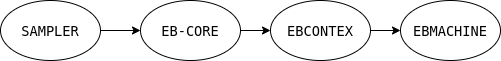
\includegraphics[scale = 0.5]{images/E2M1.png}
    \caption{Interaction between system modules}
    \label{fig:E2M1}
\end{figure}

The figure shows that the \texttt{EBMACHINE} module includes the \texttt{EBCONTEXT} module, \texttt{EBCONTEXT} includes \texttt{EB-CORE}, and \texttt{EB-CORE} includes  \texttt{SAMPLER}. When the translation of an Event-B model is done, the resulting specification includes the equations and rewrite rules necessary to extend $\mathscr{R}$ into $\mathscr{R}_\mathscr{M}$. Therefore, the system module that represents the translated Event-B model, must include the \texttt{EBMACHINE} module, which also includes all the other mentioned modules. In the end, the interaction between these modules, represent the rewrite theory $\mathscr{R}_\mathscr{M}$, as seen in the Figure \ref{fig:E2M2}.
\begin{figure}[h]
    \centering
    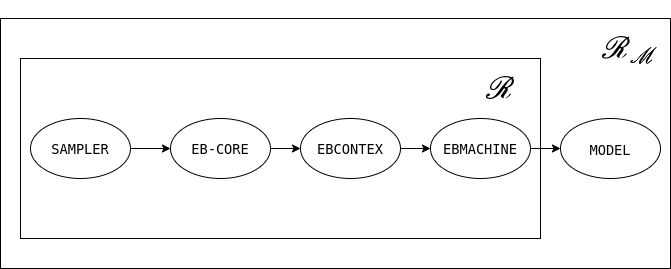
\includegraphics[scale = 0.5]{images/E2M2.png}
    \caption{Interaction between $\mathscr{R}$ and the translated model}
    \label{fig:E2M2}
\end{figure}
Using this framework for representing Event-B models in Maude, it is possible to define the complete encoding $\llbracket \cdot \rrbracket$. To guide the reader through the complete encoding, the example of the probabilistic brake system in section 2.3, Figure \ref{fig:brake3}, will be used. For the following sections, a \textit{map} will be defined as a set of pairs of the form $(x_1 \mapsto y_1, x_2 \mapsto y_2, ... , x_n \mapsto y_n)$

\section{Step 1: Encoding Contexts}
Let $\mathscr{C}$ be a context. The corresponding encoding of $\mathscr{C}$ in $\mathscr{R}$ corresponds to the term:
    \begin{align*}
    \langle \ \llbracket \mathscr{C} \rrbracket_{id} : Context \ | \ sets: \llbracket \mathscr{C} \rrbracket_{sets} , \ constants: \llbracket \mathscr{C} \rrbracket_{constants} \ \rangle
    \end{align*}   
Where $\llbracket \mathscr{C} \rrbracket_{id}$ encodes the context's identifier, $\llbracket \mathscr{C} \rrbracket_{sets}$ encodes the context's deferred sets, and $\llbracket \mathscr{C} \rrbracket_{constants}$ encodes the context's constants. The resulting term has sort \texttt{CONFIGURATION}, and represents an object of the class \texttt{Context}, with attributes \texttt{sets} and \texttt{constants}. For the probabilistic brake system, the resulting term would be the following:
\begin{maude}

<'ctxBrakeSystem: Context | 
                  sets: ('SBRAKE |-> (elt("applied"), elt("released")), 
                         'SPEDAL |-> (elt("down"), elt("up"))),
                  constants: ('MAXWEAR |-> val(elt(10))) >
\end{maude}
\begin{itemize}
    \item $\llbracket \mathscr{C} \rrbracket_{id}$ returns the identifier of the context as a a \textit{quoted identifier} \cite{MaudeManual}, which is a predefined string in Maude that is used to identify objects. In the brake model, $\llbracket \mathscr{C} \rrbracket_{id} = $\texttt{'ctxBrakeSystem}
    \item $\llbracket \mathscr{C} \rrbracket_{constants}$ returns a map of quoted identifiers, that represent the constants' names, with a term of the sort \texttt{EBType}, that represents the values of the constants. This sort functions as a wrapper for all the possible types in a Event-B model, i.e. sets, relations and basic data types. These basic data types are defined with the sort \texttt{EBElt}, that also functions as a wrapper for integers, boolean values and identifiers (represented as strings).  In the brake model, $\llbracket \mathscr{C} \rrbracket_{constants} = $ \texttt{('MAXWEAR |-> val(elt(10)))}.
    
    \item $\llbracket \mathscr{C} \rrbracket_{sets}$ returns a map of quoted identifiers, that represent the deferred sets' names, with a set of sort \texttt{EBSet}, that represent the possible values of the deferred set. The sort \texttt{EBSet} is defined as a Maude set, where the elements of the set are of sort \texttt{EBElt}. For example, in the brake model the deferred set that contains the possible states for the \textit{pedal} variable, is represented by the pair \texttt{'SPEDAL |-> (elt("down"), elt("up")))}.
\end{itemize}

\section{Step 1: Machine Initialization in Maude}
Let $\mathscr{M}$ be a probabilistic machine. The corresponding encoding of the initialization of $\mathscr{M}$ in $\mathscr{R}$ is the term:
    \begin{align*}
    & \langle \ \llbracket \mathscr{M} \rrbracket_{id} : Machine \ | \ variables: \llbracket \mathscr{M} \rrbracket_{initVars} \ \rangle 
    \end{align*}
Where $\llbracket \mathscr{M} \rrbracket_{id}$ encodes the machine's identifier and $\llbracket \mathscr{M} \rrbracket_{initVars}$ encodes the model's variables to their initial values, defined by the \textit{Init} event. The resulting term has sort \texttt{CONFIGURATION}, and represents an object of the class \texttt{Machine}, with attribute \texttt{variables}. For the probabilistic brake system, the resulting term: would be the following:

\begin{maude}

<'BrakeSystem: Machine | variables: ('brake |-> val(elt("released")), 
                                     'pedal |-> val(elt("up")), 
                                     'wear |-> val(elt(0))) >
\end{maude}

\begin{itemize}
    \item $\llbracket \mathscr{M} \rrbracket_{id}$ returns the identifier of the machine as a a quoted identifier. In the brake model, $\llbracket \mathscr{M} \rrbracket_{id} = $\texttt{'BrakeSystem}.
    \item $\llbracket \mathscr{M} \rrbracket_{initVars}$ returns a map of quoted identifiers, that represent the names of the variables, with a term of sort \texttt{EBType}, that represent the values of the variables. For example, in the brake model the variable \textit{pedal} and its value in the initial state, are represented by the pair \texttt{'pedal |-> val(elt("up"))}.
\end{itemize}

\section{Step 1: Events' States in Maude}
In order to simulate the behavior of probabilistic Event-B in Maude, it is necessary to have a deterministic method to choose the next event that is going to be executed during simulation. To do this, it is necessary to define a structure that contains the states of the events in each system configuration. These possible event's states are:
\begin{itemize}
    \item \textbf{\textit{unknown}:} the event's guards have not been evaluated.
    \item \textbf{\textit{enabled(n)}:} the event's guard is true with weight $n$.
    \item \textbf{\textit{blocked}:} the event's guard is false.
    \item \textbf{\textit{execute}:} the event has been chosen for execution in the next system transition.
\end{itemize}
This structure maps each one of the events of the model to their corresponding event state in a given system configuration. Therefore, it allows to check after each system transition the states of the events. In the meantime, this section focuses on how this structure is initialized, but the use for this structure will be detailed in the following sections.

Let $\mathscr{M}$ be a probabilistic machine. The corresponding encoding of the initialization of the events' states in $\mathscr{R}$ is the term:
    \begin{align*}
    & \langle \ events : Events \ | \ state :  \llbracket \mathscr{M} \rrbracket_{initEvtSt}  \ \rangle
    \end{align*}
Where $\llbracket \mathscr{M} \rrbracket_{initEvtSt}$ encodes the initialization of the event's states. The resulting term has sort \texttt{CONFIGURATION}, and represents an object of the class \texttt{Events}, with attribute \texttt{state}. $\llbracket \mathscr{M} \rrbracket_{initEvtSt}$ returns a set $ev(evt_1,st_1), ..., ev(evt_n,st_n)$ where each $evt_i$ is a quoted identifier that represents the name of the event, and $st_i$ is a term of sort \texttt{EvState}, that represents the state of the event. In this case, all of the $st_i = \texttt{unknown}$ , since in the initialization of the model none of the guards of the event have been evaluated. For the brake system, the resulting term after the encoding would be:
\begin{maude}

< events : Events | state: (ev('PushPedal, unknown) 
                            ev('ReleasePedal, unknown) 
                            ev('ApplyBrake, unknown) 
                            ev('ApplyBrakeFailure, unknown) 
                            ev('ReleaseBrake, unknown)) >
\end{maude}

\section{Step 1: Initial State and System States in Maude}
As seen in the preliminaries chapter, the states of the specification of a system in Maude, are represented using terms. For the translated models from probabilistic Event-B models, the initial system state of the system is:
\begin{align*}
        &\langle \ \llbracket \mathscr{C} \rrbracket_{id} : Context \ | \ sets: \llbracket \mathscr{C} \rrbracket_{sets} , \ constants: \llbracket \mathscr{C} \rrbracket_{constants} \ \rangle \\
        & \langle \ \llbracket \mathscr{M} \rrbracket_{id} : Machine \ | \ variables: \llbracket \mathscr{M} \rrbracket_{initVars} \ \rangle \\
        & \langle \ events : Events \ | \ state :  \llbracket \mathscr{M} \rrbracket_{initEvtSt}  \ \rangle
\end{align*}
This term has sort \texttt{CONFIGURATION}, and combines the previously explained objects. To refer to this term, the following notation will be used:
    \begin{align*}
        \mathfrak{C} \ \mathfrak{M}_{0}  \ \mathfrak{E}
    \end{align*}
Where $\mathfrak{C}$ is the term that represents the context, $\mathfrak{M}_{0}$ is the term that represents the machine in the initial state, and $\mathfrak{E}$ is the term that represents the events' states in the current system configuration. The rest of the system states, are symbolized with $\mathfrak{C} \ \mathfrak{M}_{i}  \ \mathfrak{E}$, and are obtained with the application of equations and rewrite rules, defined in $\mathscr{R}_\mathscr{M}$,  over the initial state $\mathfrak{C} \ \mathfrak{M}_{0}  \ \mathfrak{E}$. With these elements, the definition of the rewrite theory $\mathscr{R}$ is concluded. The following sections provide the definition of the equations and rewrite rules that define $\mathscr{R}_\mathscr{M}$.

\section{Step 2: $evalSt$ Equation}
The $evalSt$ equation, determines if an event is enabled or blocked, given the current state of the machine $\mathfrak{M}_i$ and the encoding of the guards of the event $e_i$, represented as $\llbracket \mathscr{M} \rrbracket^{e_i}_{guards}$ :
\begin{align*}
    &\mathfrak{C} \ \mathfrak{M}_{i} \ \langle events : Events \ | \ state: ev(e_1,unknown) ... ev(e_n, unknown) \rangle = \\
    &\mathfrak{C} \ \mathfrak{M}_{i} \ \langle events : Events \ | \ state: ev(e_1, eval(\mathfrak{M}_i, \llbracket \mathscr{M} \rrbracket^{e_1}_{guards})) ... ev(e_n, eval(\mathfrak{M}, \llbracket \mathscr{M} \rrbracket^{e_n}_{guards})) \rangle
\end{align*}
To do this, for each one of the event states $ev(evt_1,st_1), ..., ev(evt_n,st_n)$, the equation evaluates the new state of the event $e_i$ with the equation $eval$. The equation takes as input the current state of the machine $\mathfrak{M}_i$, i.e. the value of each one of the variables, and then determines if the guards of event $e_i$ are satisfied, using the encoded version of the guards  $\llbracket \mathscr{M} \rrbracket^{e_n}_{guards}$. The returned value by $eval$, can only be \texttt{enabled(n)}, if the guards of the event are satisfied in $\mathfrak{M}_i$, or \texttt{blocked} otherwise. For example, if $evalSt$ is applied to the first state $\mathfrak{C} \ \mathfrak{M}_{0}  \ \mathfrak{E}$, the obtained term is:
\begin{maude}

$\mathfrak{C}$ $\mathfrak{M}_0$ < events : Events | state: (ev('PushPedal, enable(10)) 
                                 ev('ReleasePedal, blocked) 
                                 ev('ApplyBrake,blocked) 
                                 ev('ApplyBrakeFailure, blocked)
                                 ev('ReleaseBrake, blocked)) >
\end{maude}



\section{Step 2: $chooseEvt$ Rule}
The $chooseEvt$ rule chooses probabilistically, the next event to be executed according to the weights of the enabled events:
\begin{align*}
    \mathfrak{C} \ \mathfrak{M}_i \ \langle state: ev(e_1,st_1) ... ev(e_n, st_n) \rangle \rightarrow 
    \mathfrak{C} \ \mathfrak{M}_i \ \langle state: ev(e_i, execute) \rangle
\end{align*}
To do this, the following steps must be applied:
\begin{enumerate}
    \item Filter out the events $ev(e_i, st_i)$ where $st_i = \texttt{blocked}$. Thus, the remaining set of event states will have the form $ev(e_j, enabled(n_j)),...,ev(e_k, enabled(n_k))$.
    \item From the enabled events, choose probabilistically one of the events $e_i$, according to their weights $n_j...n_k$, as done in probabilistic Event-B.
    \item The chosen event $e_i$ is paired with the state \texttt{execute}, and the resulting set of event states is $ev(e_i, execute)$.
\end{enumerate}
For example, if the rule is applied to the following state from the brake example:
\begin{maude}

$\mathfrak{C} \ \mathfrak{M}_i$ <events : Events | state: ev('PushPedal, blocked) 
                               ev('ReleasePedal, enabled(10)) 
                               ev('ApplyBrake,enabled(7)) 
                               ev('ApplyBrakeFailure, enabled(3))
                               ev('ReleaseBrake, blocked)>
\end{maude}
The resulting term with the highest probability is:
\begin{maude}

$\mathfrak{C} \ \mathfrak{M}_i$ <events : Events | state : ev('ReleasePedal, execute)>
\end{maude}
Since the \textit{ReleasePedal} event has the biggest weight.

\section{Step 2: $execEvt_{e_i}$ Rule}
For each one of the events $e_i$ in the original probabilistic Event-B model, a rule $execEvt_{e_i}$ is encoded. It is defined as: 
\begin{align*}
    \mathfrak{C} \ \mathfrak{M}_i \ \langle state: ev(e_i, execute) \rangle \rightarrow \mathfrak{C} \ \mathfrak{M}_j \ \langle state: \llbracket \mathscr{M} \rrbracket_{initEvtSt} \rangle
\end{align*}
where $\mathfrak{M}_j$ is obtained by changing the variable values according to the encoded probabilistic assignments of the specific event $e_i$. Furthermore, after making the system transition from $\mathfrak{M}_i \rightarrow \mathfrak{M}_j$, the states of the events are reseted to \texttt{unknown}, as done in the initialization of the model.
For example, if the current state is:
\begin{maude}

$\mathfrak{C}$ <'BrakeSystem: Machine | variables: ('brake |-> val(elt("released")), 
                                        'pedal |-> val(elt("up")), 
                                        'wear |-> val(elt(0))) >
  <events : Events | state: ev('PushPedal, execute) >
\end{maude}
After executing rule $execEvt_{PushPedal}$ the resulting state with highest probability is:
\begin{maude}

$\mathfrak{C}$ <'BrakeSystem: Machine | variables: ('brake |-> val(elt("released")), 
                                        'pedal |-> val(elt("down")), 
                                        'wear |-> val(elt(0))) >
  < events : Events | state: (ev('PushPedal, unknown) 
                              ev('ReleasePedal, unknown) 
                              ev('ApplyBrake, unknown) 
                              ev('ApplyBrakeFailure, unknown) 
                              ev('ReleaseBrake, unknown)) >
\end{maude}
Since the \textit{down} value for the \textit{pedal} variable, has a $90\%$ chance of being selected, in the probabilistic assignment from the original model.

\section{$\mathscr{R}_\mathscr{M}$ in a Nutshell}
Using all the previously explained elements of the rewrite theory $\mathscr{R}_\mathscr{M}$, it is possible to summarize how the encoding produces a rewrite theory, that has the same behavior of a probabilistic Event-B model: 


\begin{enumerate}
    \item The probabilistic Event-B is encoded to the rewrite theory $\mathscr{R}_\mathscr{M}$, using $\llbracket \cdot \rrbracket$:
    \begin{align*}
        \llbracket \cdot \rrbracket: (\mathscr{C}, \mathscr{M}) \rightarrow \mathscr{R}_\mathscr{M}
    \end{align*}
    \item The system is initialized with term $\mathfrak{C \ M_0 \ E}$ inside $\mathscr{R}_\mathscr{M}$:
    \begin{align*}
        \mathfrak{C \ M_0 \ E}
    \end{align*}
    \item For any state of the model, symbolized by $\mathfrak{M_i}$, the event guards are evaluated using the equation $evalSt$.
    \begin{align*}
        \mathfrak{C \ M_i} \ \langle state: ev(e_1,unknown) ... ev(e_n, unknown) \rangle \xrightarrow{evalSt} \mathfrak{C \ M_i} \ \langle state: ev(e_1,st_1) ... ev(e_n, st_n) \rangle
    \end{align*}
    \item The blocked events are filtered and the next event is chosen probabilistically from all the enabled events, based on the event's weights:
    \begin{align*}
        \mathfrak{C \ M_i} \ \langle state: ev(e_1,st_1) ... ev(e_n, st_n) \rangle \xrightarrow{chooseEvt} \mathfrak{C \ M_i} \ \langle state: ev(e_i,execute) \rangle
    \end{align*}
    \item The rule associated to the encoded version of the chosen event $e_i$ in the previous step is executed. The resulting change of the variable values, is captured in the rewrite $\mathfrak{M_i} \rightarrow \mathfrak{M_j}$. Moreover, the states of the events are initialized again. 
    \begin{align*}
        \mathfrak{C \ M_i} \ \langle state: ev(e_i,execute) \rangle \xrightarrow{execEvt_{e_i}} \mathfrak{C \ M_j} \ \langle state: ev(e_1,unknown) ... ev(e_n, unknown) \rangle
    \end{align*}
    \item Repeat steps 3,4 and 5 until deadlock (i.e. none of the events can be executed since the guards of the events are unsatisfiable), or until the rule $execEvt_{e_i}$ has been executed a fixed number of times (this value is represented as a constant named \texttt{MAX-STEPS} inside $\mathscr{R}_\mathscr{M}$).
\end{enumerate}
Based on the presented encoding, it is possible to prove that the resulting rewrite theory $\mathscr{R}_\mathscr{M}$ is semantically correct, based on the probabilistic Event-B model $(\mathscr{C}, \mathscr{M})$:

\begin{theorem}[adequacy]
Let $(\mathscr{C}, \mathscr{M})$ be an Event-B model and
$\mathcal{R}_{\mathcal{M}}$ be a rewrite theory obtained by the encoding $\llbracket \cdot \rrbracket: (\mathscr{C}, \mathscr{M}) \rightarrow \mathscr{R}_\mathscr{M}$. Furthermore, let $s$ and $s'$ be states or configurations of $\mathscr{M}$ (i.e. valuations of the variables in $\mathscr{M}$), and $s \xRightarrow{e_i,p} s'$ be a system transition from state $s$ to $s'$, using the event $e_i$ with probability $p$. Then $s \xRightarrow{e_i,p} s'$ iff $\llbracket \mathscr{M} \rrbracket_s \rightarrow_p \llbracket \mathscr{M} \rrbracket_{s'}$, where $\llbracket \mathscr{M} \rrbracket_s$ and $\llbracket \mathscr{M} \rrbracket_{s'}$ correspond to the encoded version of states $s$ and $s'$ respectively, and $\rightarrow_p$ denotes one-step rewriting in $\mathscr{R}_\mathscr{M}$ with probability $p$.
\end{theorem}

\textbf{\textit{Proof.}} The reader can refer to \cite{Olarte} for the proof sketch of this theorem $\square$.